\scanpage{5}

de fractions $K$, on peut \unsure{prouver|penser} que les sous-algèbres $\mathcal A$ de $\operatorname{Et}(X,\Lambda)$ ainsi obtenues sont les traces sur $\operatorname{Et}(X,\Lambda)$ des sous-algèbres de $\operatorname{Et}(X,\Lambda)\otimes_\Lambda K\simeq\operatorname{Et}(X,K)$ [i.e. satisfaisant la condition que si $\varphi\in\operatorname{Et}(X,\Lambda)$ \deleted{est} et $\lambda\in\Lambda$ \deleted{$\unsure{\ne0}$} sont tels que $\lambda\ne0$ et $\lambda\varphi\in\mathcal A$, alors $\varphi\in\mathcal A$]

\figure{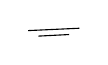
\begin{tikzpicture}[x=1cm,y=1cm]\draw (0,0)--(0.65,0.03);\draw (0.13,-0.07)--(0.52,-0.05);\end{tikzpicture}}

Nous supposons maintenant que $X$ est un espace topologique, et considérons la condition
\[
\text{c)}\quad\forall A\in F,\quad\text{on a}\quad\overline A\in F
\]
équivalente (moyennant a)) à
\[
\text{c')}\quad\forall A\in F,\quad\text{on a}\quad A^\circ\in F.
\]
Ceci implique donc que
\[
\dot A=\overline A-A^\circ\ \deleted{\text{est}}\ \in F
\]
donc la \inserted{\unsure{prem.}} partition de $X$ en $A^\circ$, $\unsure{(\complement A)^\circ}=X-\overline A$, $\dot A$ est formée d'éléments de $F$.

\deleted{d) $\forall A\in F$, \inserted{\deleted{\unsure{A}} tel que $A$ loc. fermé i.e. $\overline A-A$ fermé, (i.e. $A=B-C$ pour $B,C\in F$)} \deleted{$A$ est localement connexe, et les} \deleted{\unsure{les}} composantes connexes sont \inserted{ouvertes, de nb fini et} $\in F$.}

\mspage{6}
